\documentclass[11pt]{article}
\usepackage{a4wide}
\usepackage{times}
\usepackage[french]{babel}
\usepackage[T1]{fontenc} 
\usepackage[utf8]{inputenc}
\usepackage{url}

\usepackage{eurosym}
\usepackage{amssymb}
\usepackage{xcolor}
\newcommand{\mynote}[3][black]{\textcolor{#1}{\fbox{\bfseries\sffamily\scriptsize{#2}}
{\small$\blacktriangleright$\textsf{\emph{#3}}$\blacktriangleleft$}}}
\newcommand{\pem}[1]{} %{\mynote[cyan]{Pierre-Etienne}{#1}}
\newcommand{\ld}[1]{\mynote[magenta]{Laurence}{#1}}
\newcommand{\TODO}[1]{\mynote[red]{TODO}{#1}}
%\newcommand{\TODO}[1]{}
\newcommand{\silent}[1]{}
\newcommand{\gpl}[0]{génie de la programmation et du logiciel}
\newcommand{\eg}[0]{\emph{e.g.},~}
\newcommand{\ie}[0]{\emph{i.e.},~}
\newcommand{\etal}[0]{\emph{et al.}~}
\newcommand{\wrt}[0]{\emph{w.r.t.}~}
\newcommand{\cf}[0]{cf.~}
\usepackage{pdfpages}


\title{GdR Génie de la Programmation et du Logiciel\\ 
Défis 2030? 2026?}
\author{Mireille Blay-Fornarino, Catherine Dubois, Pierre-Etienne Moreau\\
\\
%%\textbf{DRAFT}
}
\begin{document}
\maketitle

\section{Introduction}

Le Génie de la Programmation et du Logiciel est au c{\oe}ur de l'activité
informatique. Les concepts, méthodes et les outils de conception et de
validation de logiciels constituent les éléments manipulés par les
informaticiens pour maîtriser et automatiser les problèmes qui leur sont
soumis. 
Plusieurs grandes familles thématiques ont été définies lors des actions de prospective que nous avons menées en 2010 et 2014, et qui avaient conduit à plusieurs Groupes de Travail (GT). 
Fin 2019, nous avons lancé une nouvelle action dans ce sens\footnote{\url{http://gdr-gpl.cnrs.fr/node/384}}. %Nous travaillons encore sur les retours, mais nous avons déjà identifié, les grandes thématiques suivantes, à savoir :\\

Les grandes thématiques du domaine sur lesquelles les chercheurs du
domaine travaillent sont, au regard des 21 défis reçus en décembre 2019~: 
\begin{itemize}
  \renewcommand{\labelitemi}{$\bullet$}
\item l'ingénierie dirigée par les modèles qui exploite une continuité entre  modélisation, conception, programmation et développement pour systématiser la production et la maintenance de logiciels plus sûrs et plus agiles, elle inclut~:
\begin{itemize}
\item l'ingénierie des exigences et de leurs interactions avec les artefacts logiciels pour assurer la traçabilité logicielle, y compris dans des objectifs d'argumentation et de validation de la justesse des systèmes produits, 
\item la séparation et la composition de préoccupations, par exemple la sécurité, pour maîtriser la conception, le développement et l'évolution de grands systèmes, 
\item la modélisation et la gestion de la variabilité logicielle à des fins de production, de configuration et de maintenance de lignes de produits logiciels;
\end{itemize}

\item la conception et l'outillage de langages plus sûrs et plus expressifs,  elle inclut~: 
\begin{itemize}
\item les approches de compilation pour des architectures spécifiques et notamment parallèles, y compris ces dernières années pour l'exploitation des GPU et  des ordinateurs quantiques,
\item la conception et l'utilisation de langages métiers et de langages spécifiques à des domaines,
\item la certification des chaînes de compilation,
\item de nouvelles approches de la réparation de "bugs";
\end{itemize}
%et s'appuie sur des techniques de  transformation de modèles,

\item le développement de techniques de vérification et de validation des systèmes, elle inclut~:
\begin{itemize}
\item la vérification et la validation à partir  de spécifications ou de code : analyse statique, génération de tests et raffinements prouvés,
\item la prise en compte de la testabilité logicielle de l'élaboration des systèmes logiciels à leur adaptation en production, y compris dans des contextes d'intégration d'intelligence artificielle, 
\item l'adaptation de ces travaux aux systèmes émergents tels que les systèmes cyber-physiques, les systèmes intégrant de l'IA, les véhicules autonomes;
\end{itemize}
\item la prise en compte dans l'ensemble du cycle de vie du logiciel des propriétés telles que la  sécurité, la sobriété écologique, la résilience, elle inclut~:
\begin{itemize}
\item la recherche sur de nouvelles architectures logicielles et méthodes de développements pour faire face aux nouvelles contraintes : taille des systèmes, mondialisation du développement, protection des données, gestion des ressources, déconnexion, ...
\item l'adaptation des approches de développement pour intégrer la maintenance et l'adaptation dynamique des systèmes aux changements de contexte, y compris par apprentissage automatique, en particulier pour les systèmes cyber-physiques;
\end{itemize}
\item l'étude des pratiques de développement y compris de maintenance logicielle, notamment par des études empiriques et la mise au point d'abstractions adaptées;
\item  l'exploitation des travaux sur l'IA dans un contexte de \gpl~et inversement, dont les travaux cités précédemment.

\end{itemize}

Sans vouloir être exhaustif, ces grandes thématiques regroupent une grande partie des
thèmes de la programmation et du génie logiciel abordés par les équipes
françaises actuellement. 
\noindent
Avec l'omniprésence de l'informatique dans notre vie que ce soit en termes
d'informatique embarquée, d'intelligence ambiante, d'extension du web au niveau
de la planète, d'intégration dans les objets du quotidien, ou encore avec le
développement de grandes infrastructures de calcul ou de traitement de grandes
masses de données, de nouvelles questions de recherche sont posées.
De nouveaux paradigmes, de nouveaux langages, de nouvelles approches de
modélisation, de vérification, de tests et de nouveaux outils dans le domaine
de la programmation et du logiciel devraient voir le jour dans les 5 à 10 ans à
venir, que ce soit pour faciliter la vie des concepteurs de logiciels, pour
modéliser et fiabiliser les logiciels ou encore pour devancer l'évolution
technologique, mais également pour prendre en compte de nouveaux enjeux de
société tels que le développement durable, les économies d'énergie ou la maîtrise des systèmes intégrant de l'intelligence artificielle.



\section{Defis 1}

\section{Conclusion}
\section{Références}


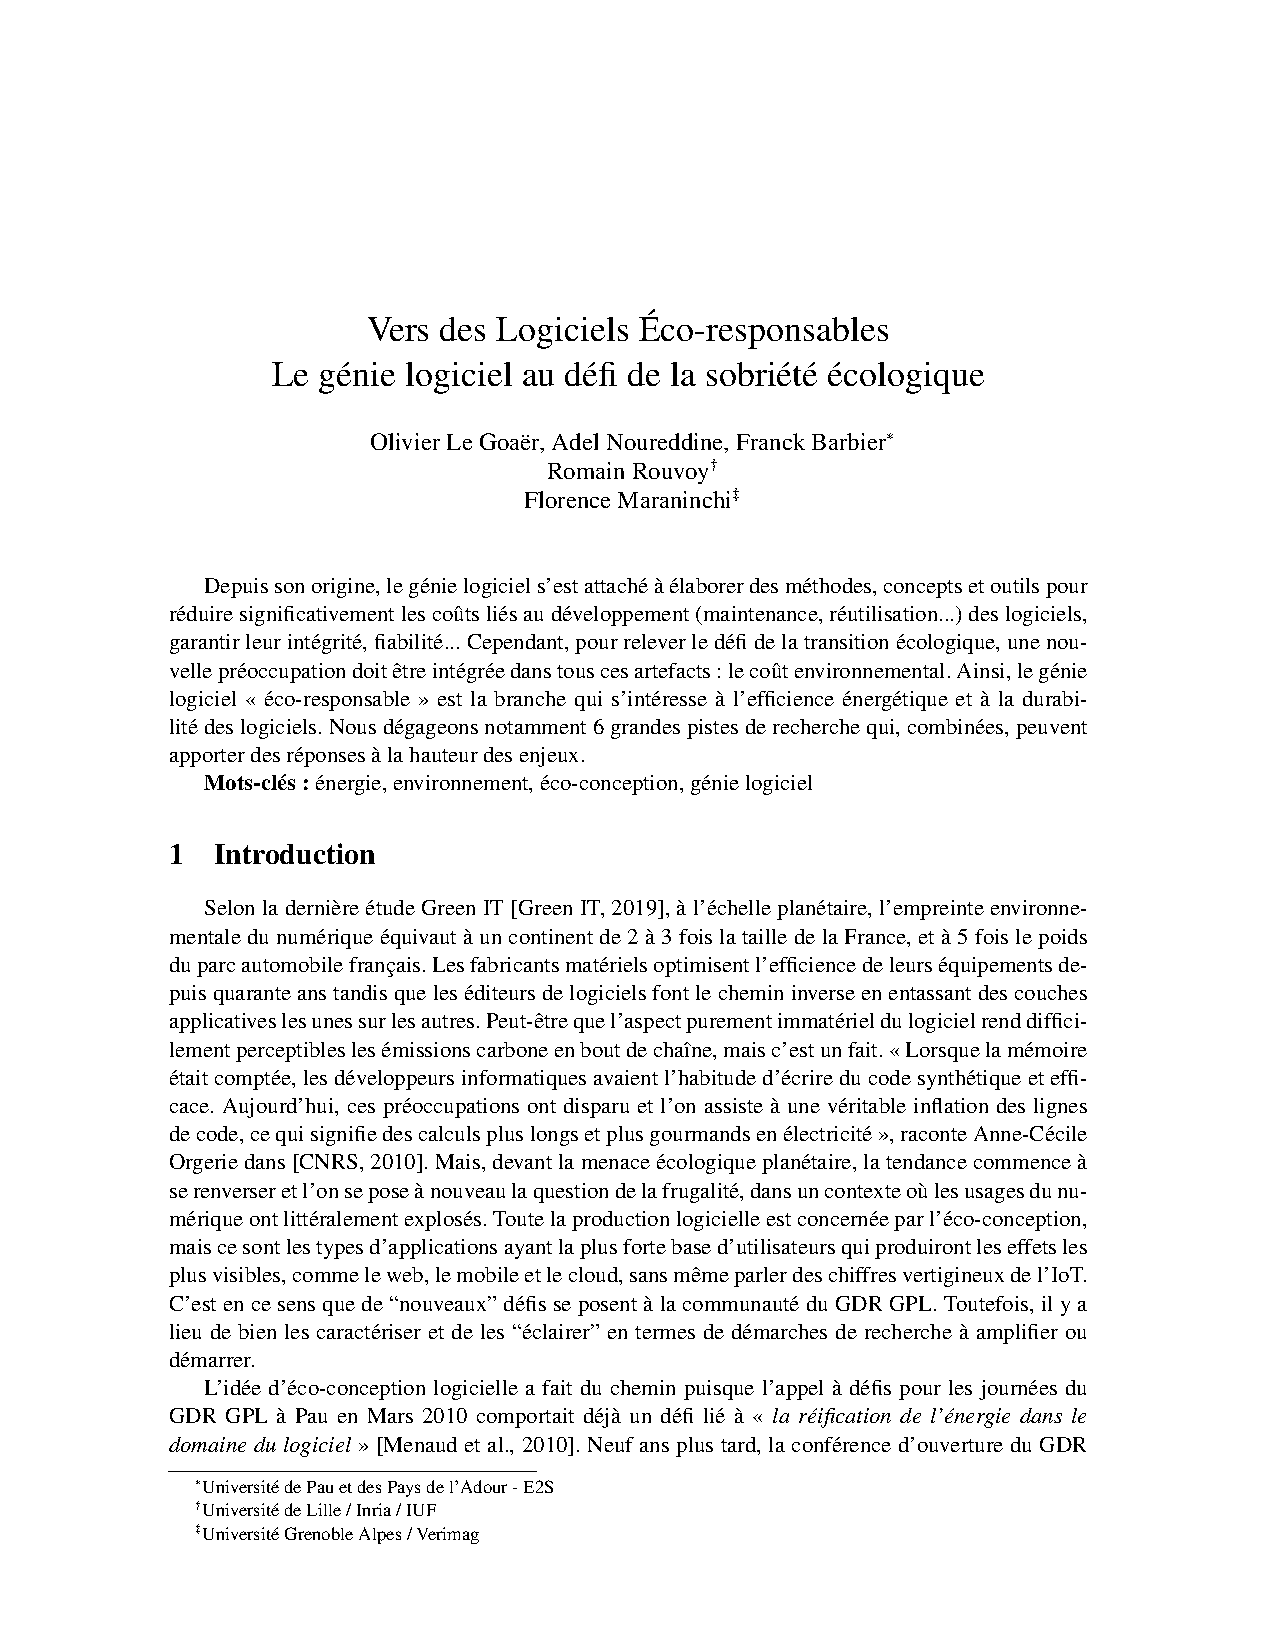
\includepdf[pages=-,pagecommand={\thispagestyle{plain}}]{Defis/logiciels_verts.pdf}

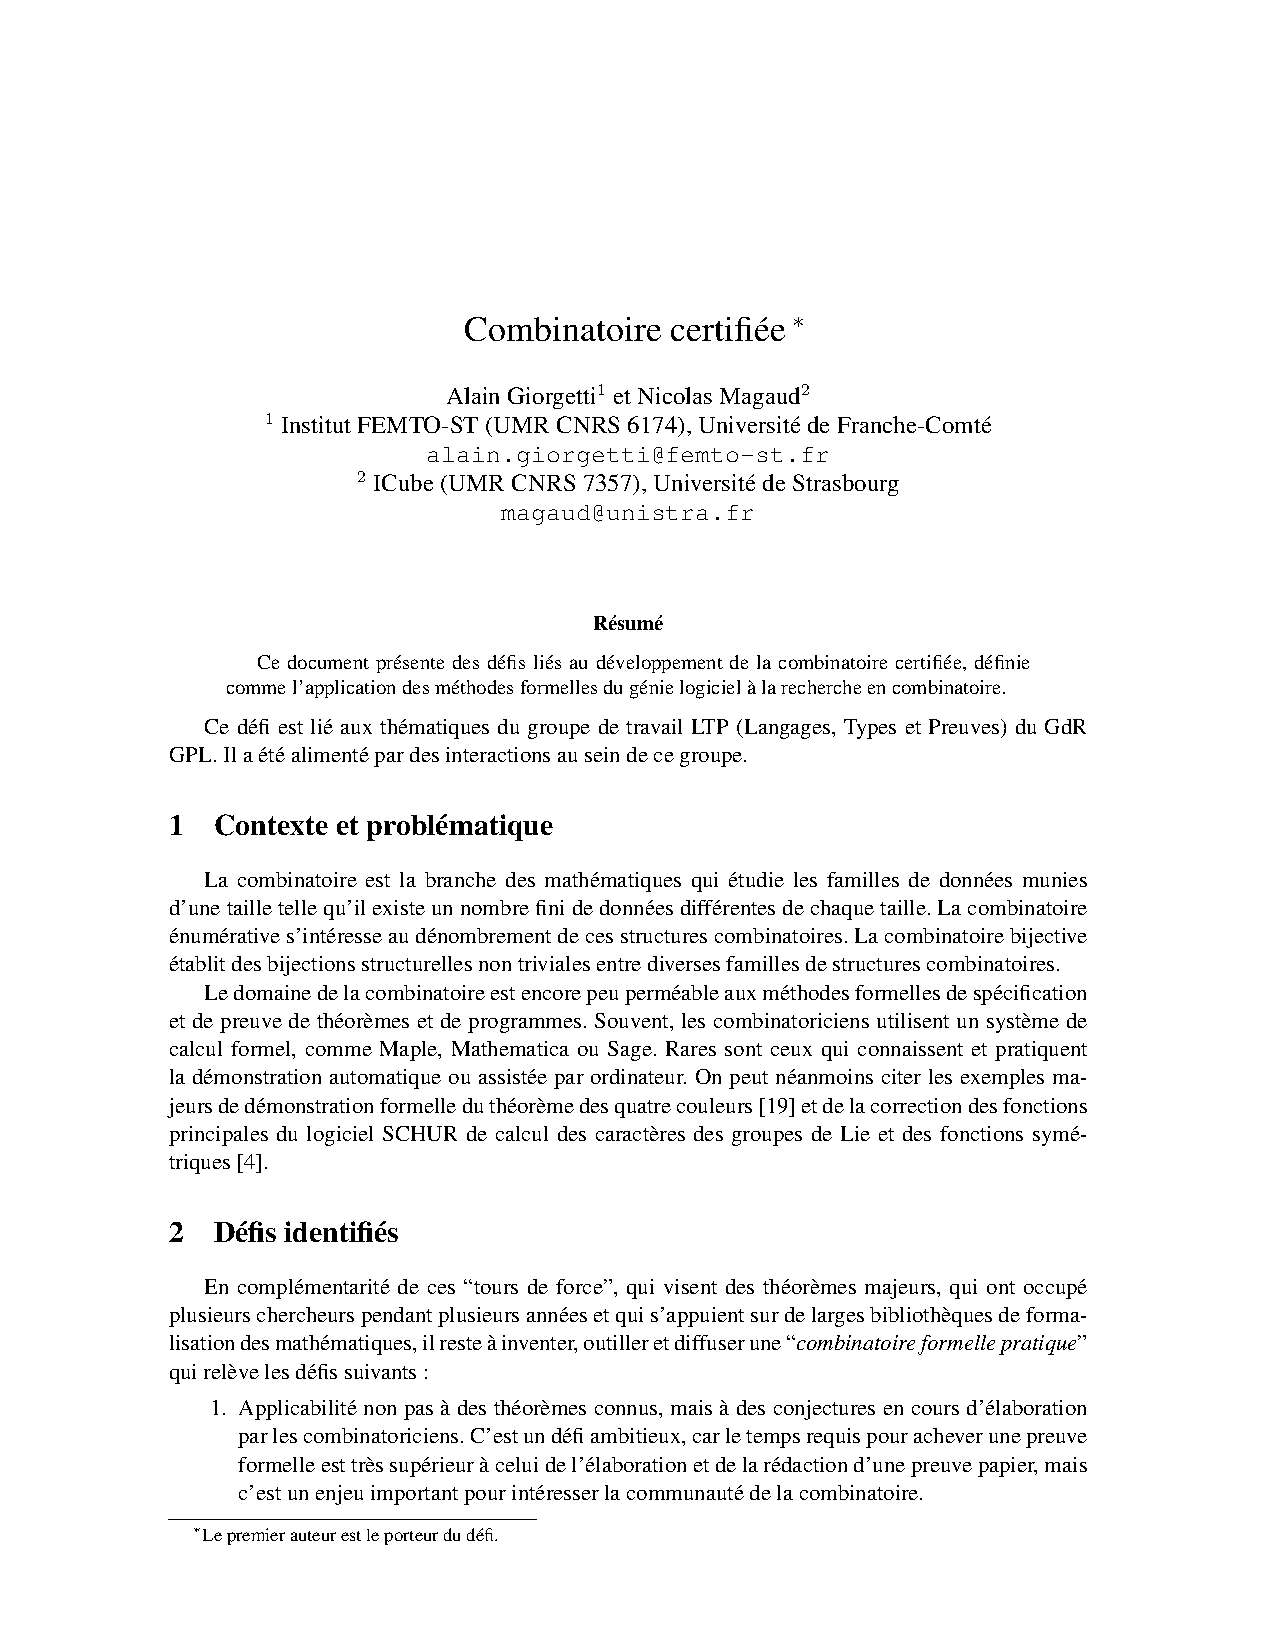
\includepdf[pages=-,pagecommand={\thispagestyle{plain}}]{Defis/combinatoire_certifiee.pdf}


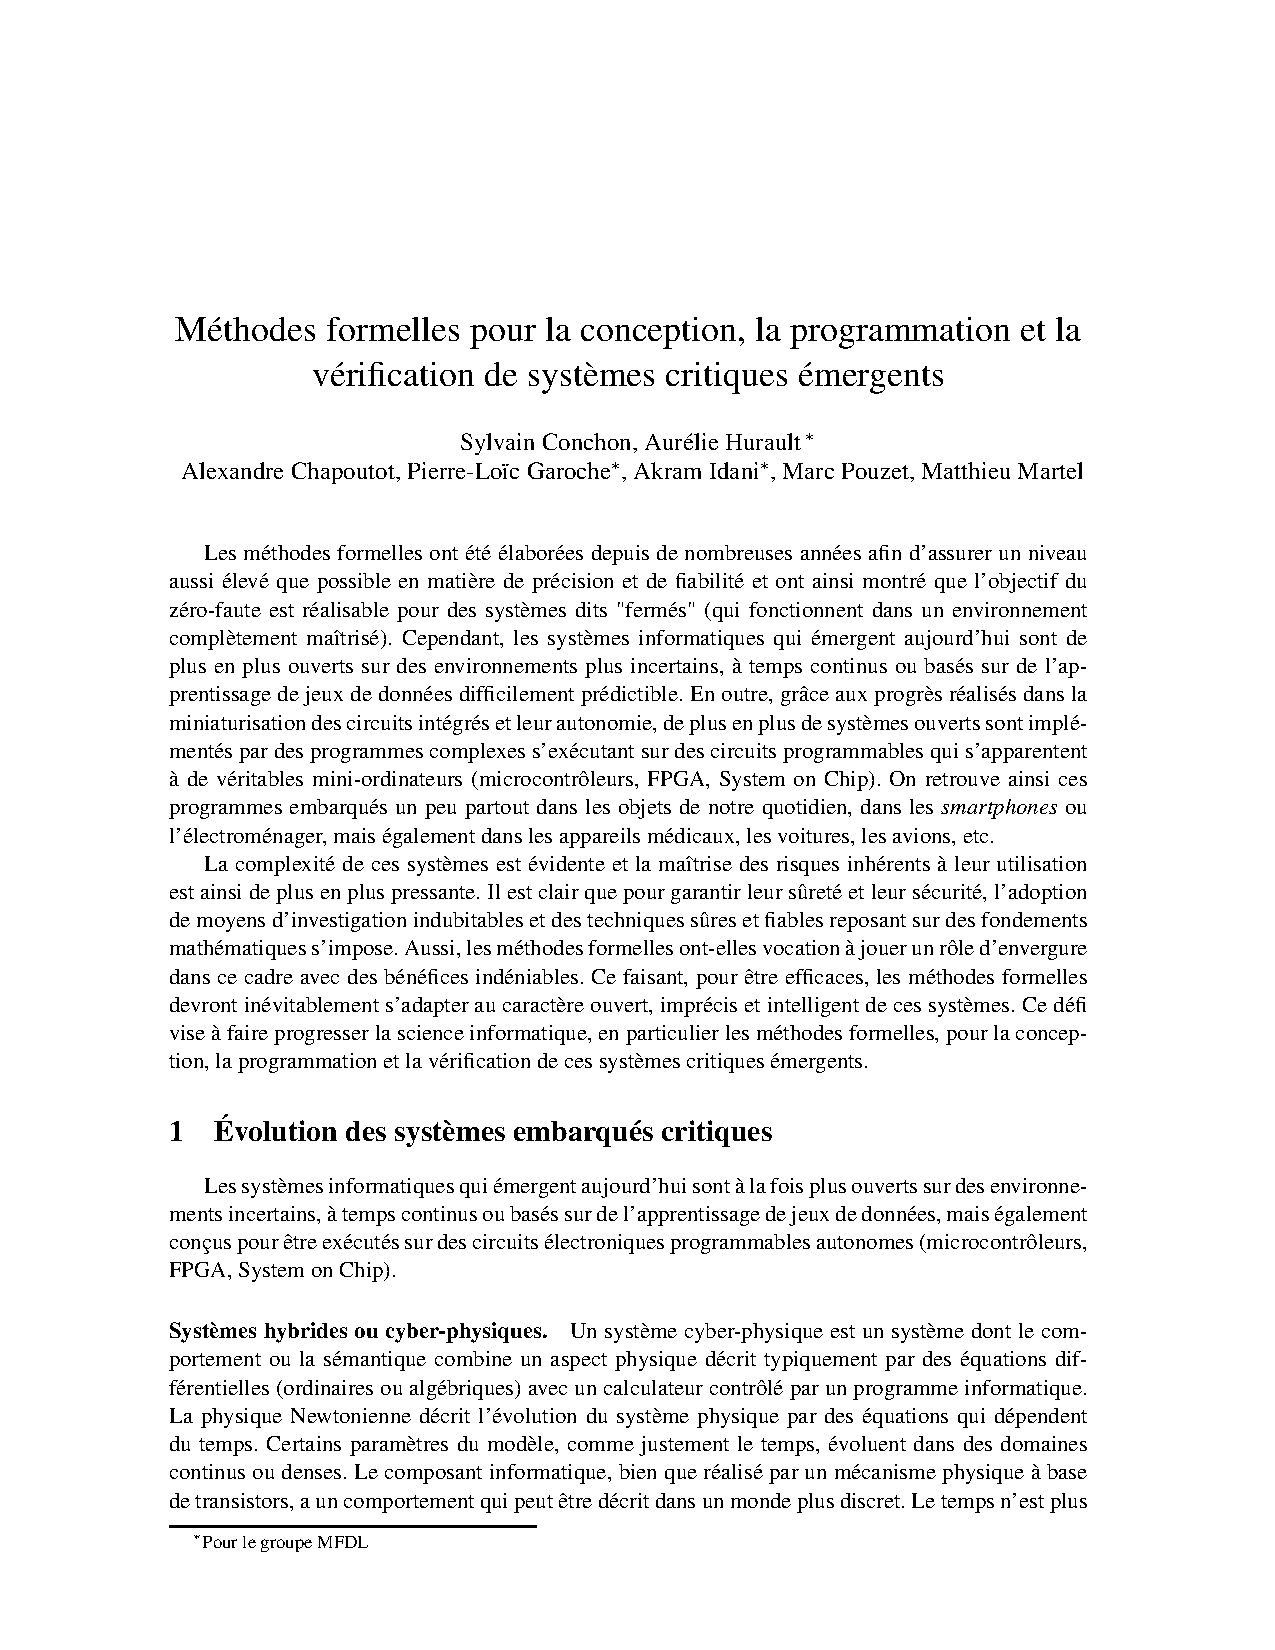
\includepdf[pages=-,pagecommand={\thispagestyle{plain}}]{Defis/FM_systemes_emergents.pdf}

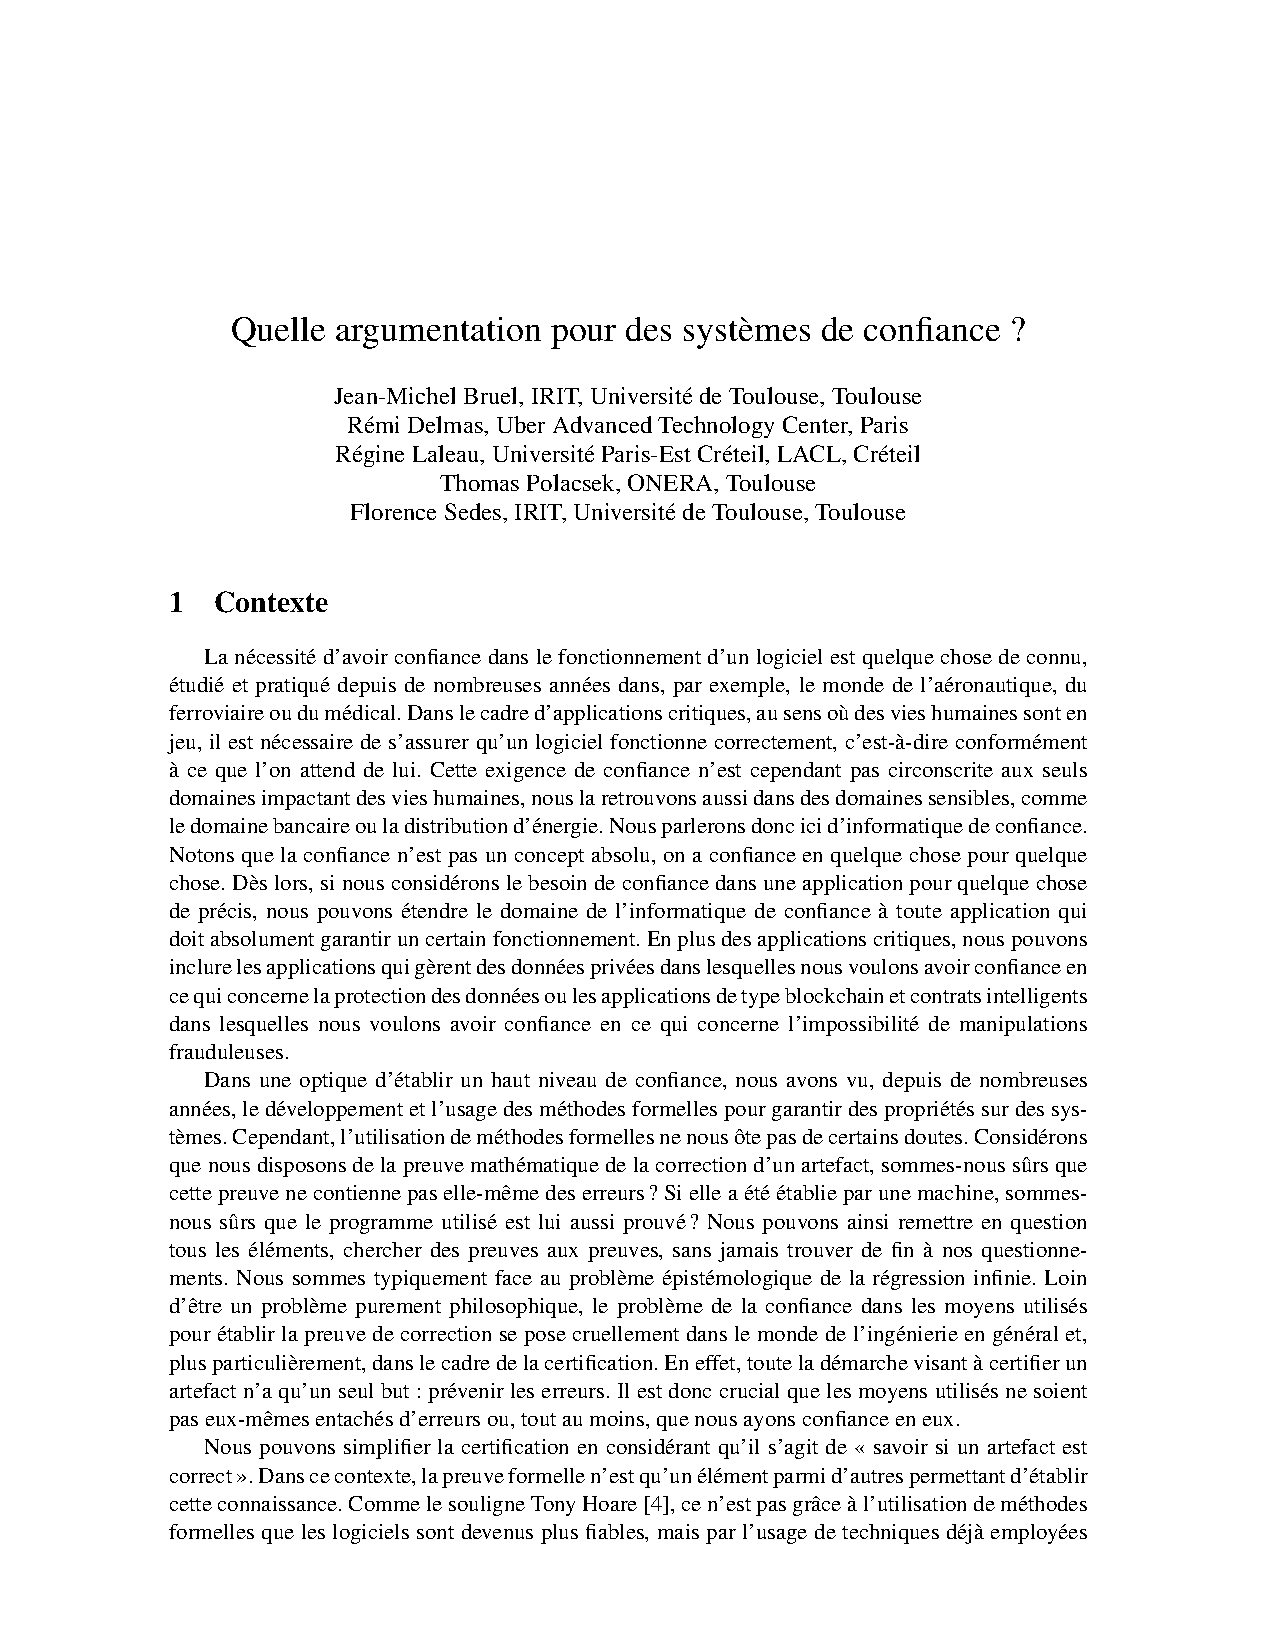
\includepdf[pages=-,pagecommand={\thispagestyle{plain}}]{Defis/argumentation_pour_des_systemes_de_confiance.pdf}
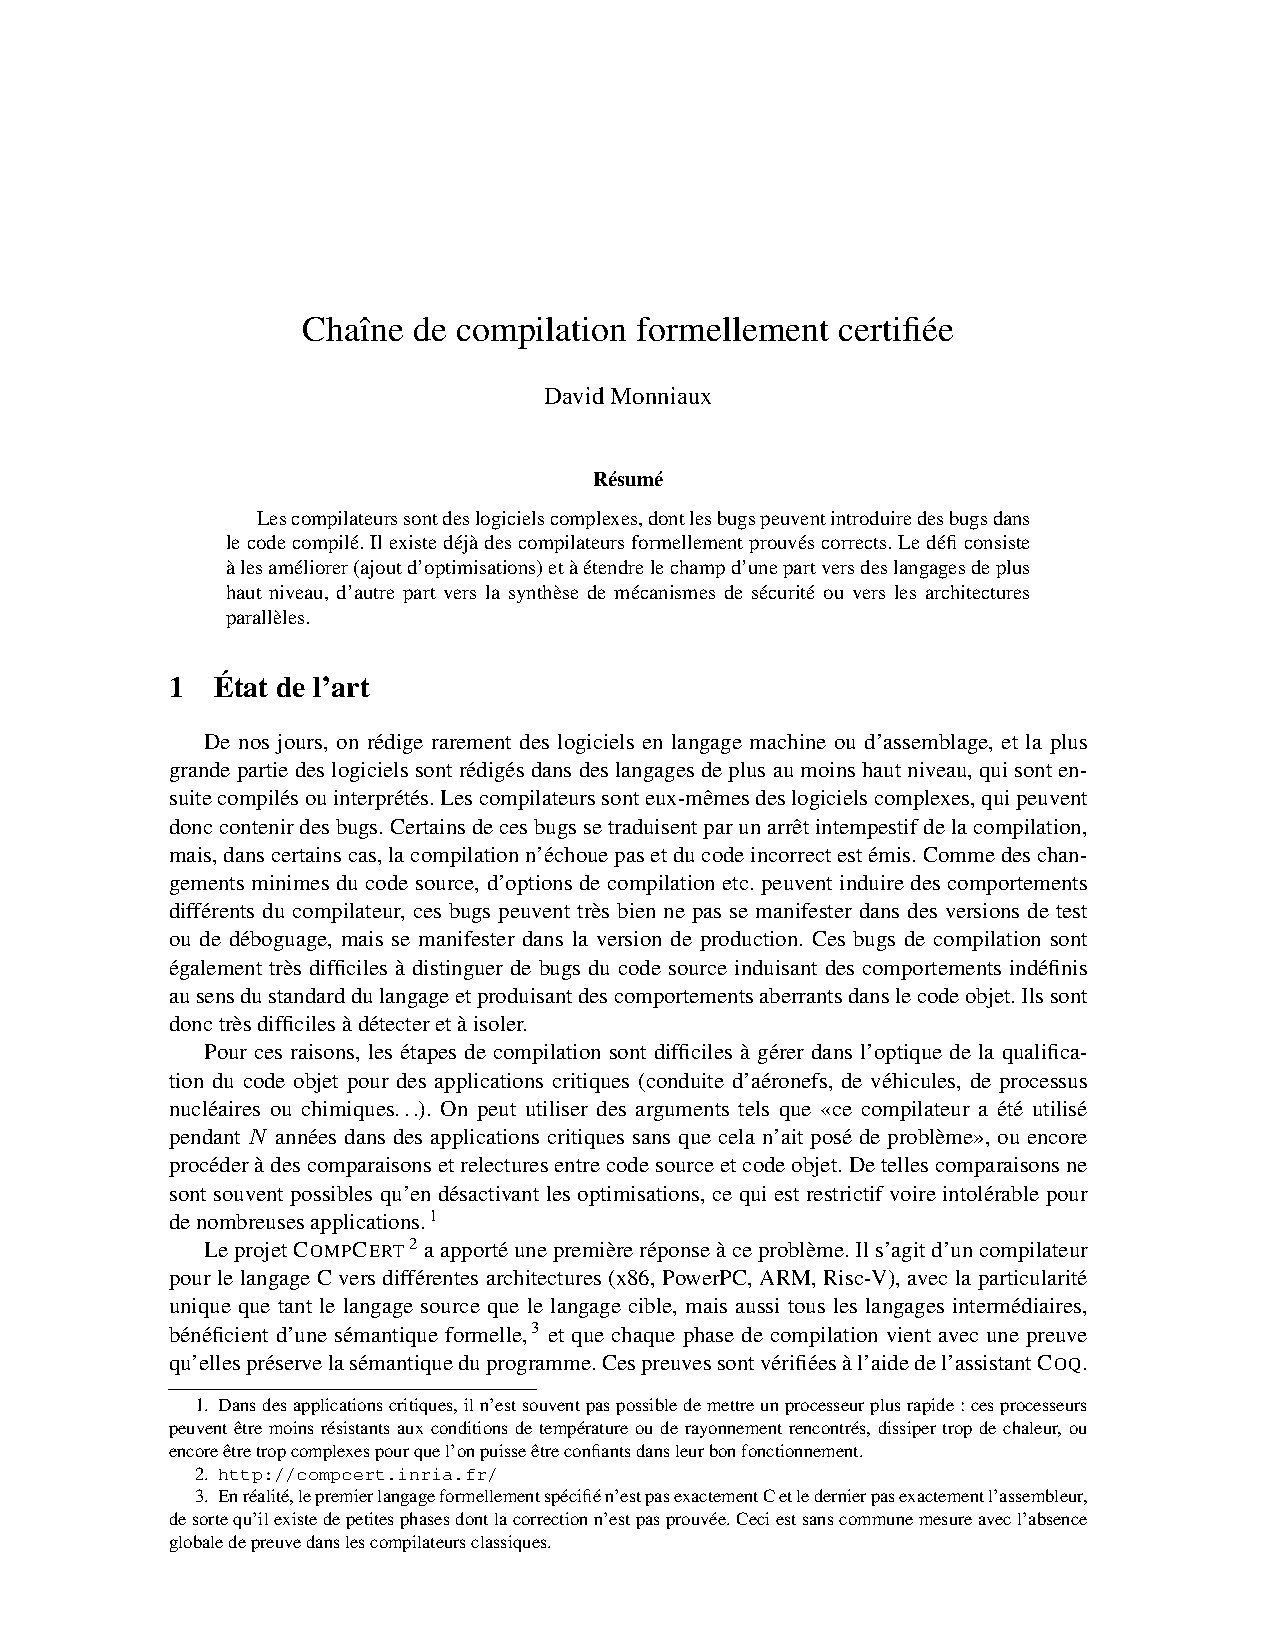
\includepdf[pages=-,pagecommand={\thispagestyle{plain}}]{Defis/chaine_compilation_certifiee.pdf}
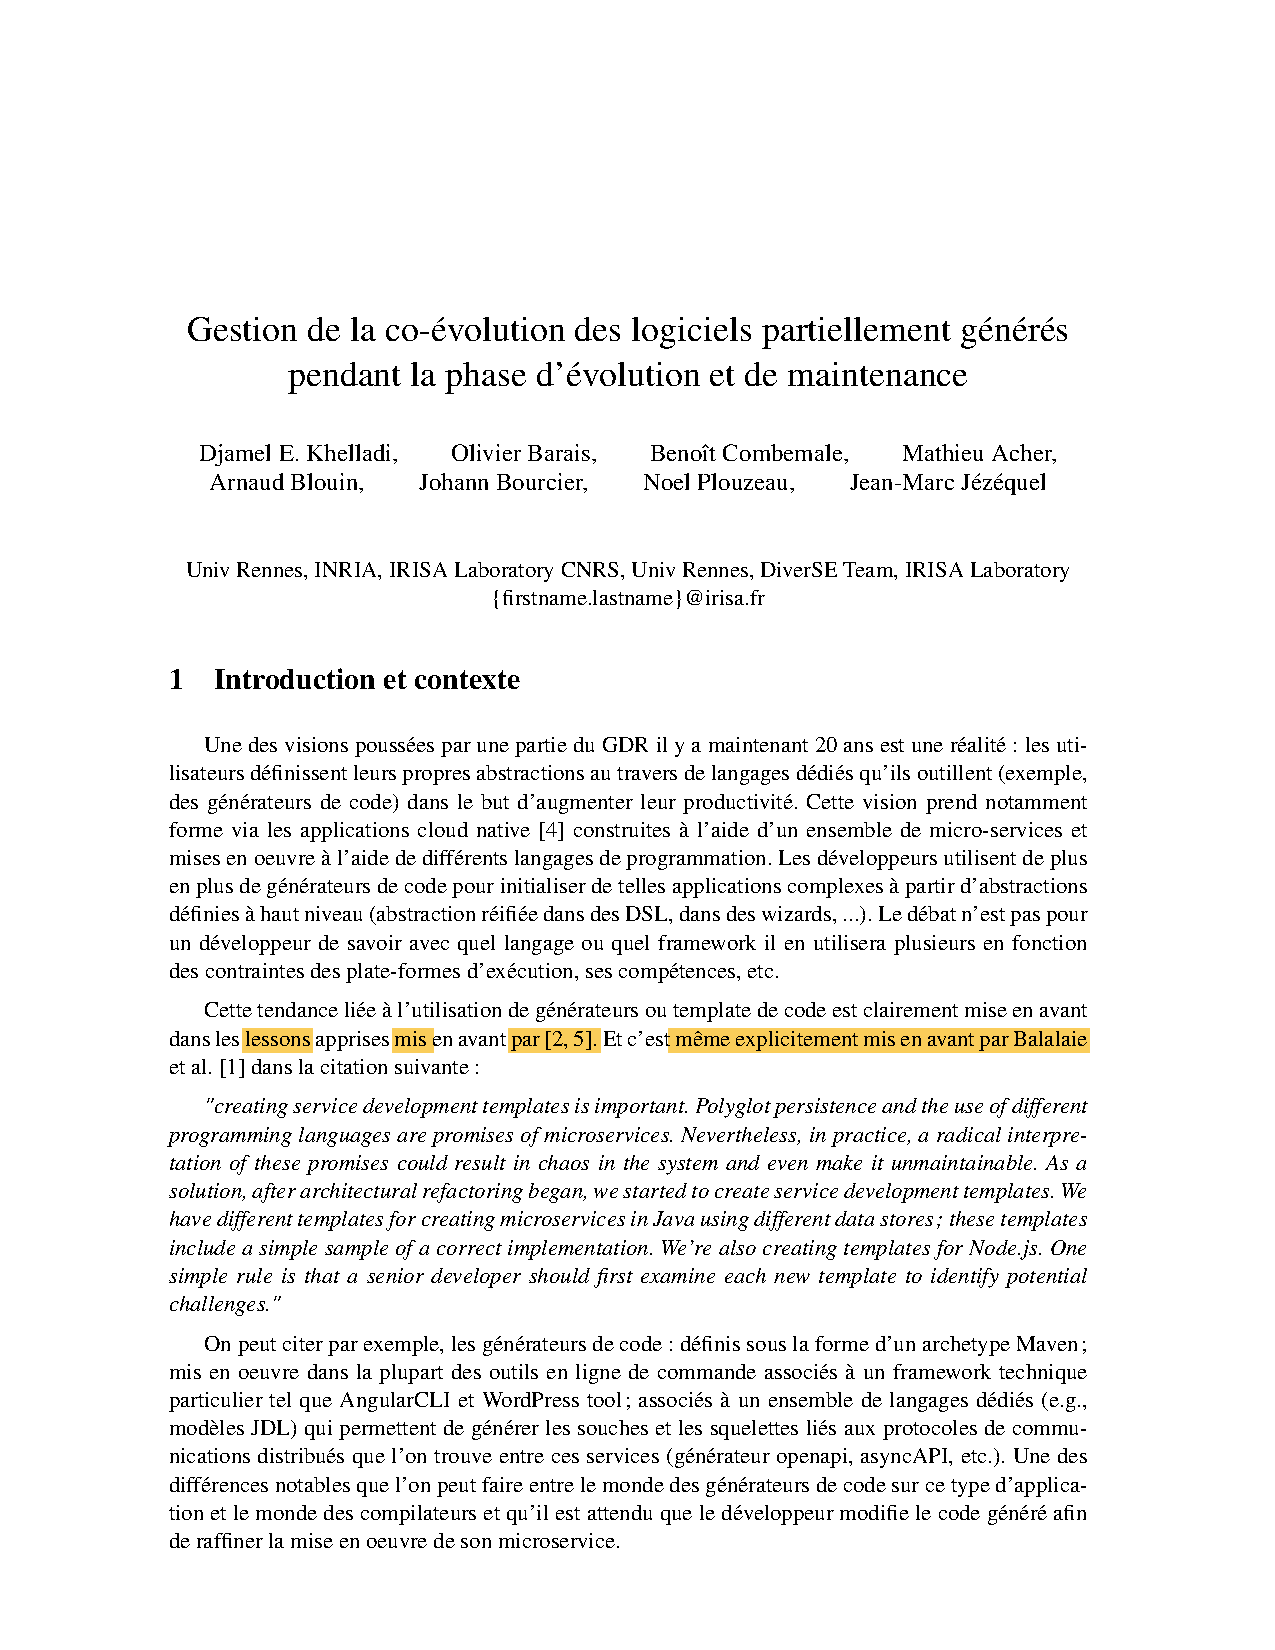
\includepdf[pages=-,pagecommand={\thispagestyle{plain}}]{Defis/co-evolution_des_logiciels.pdf}
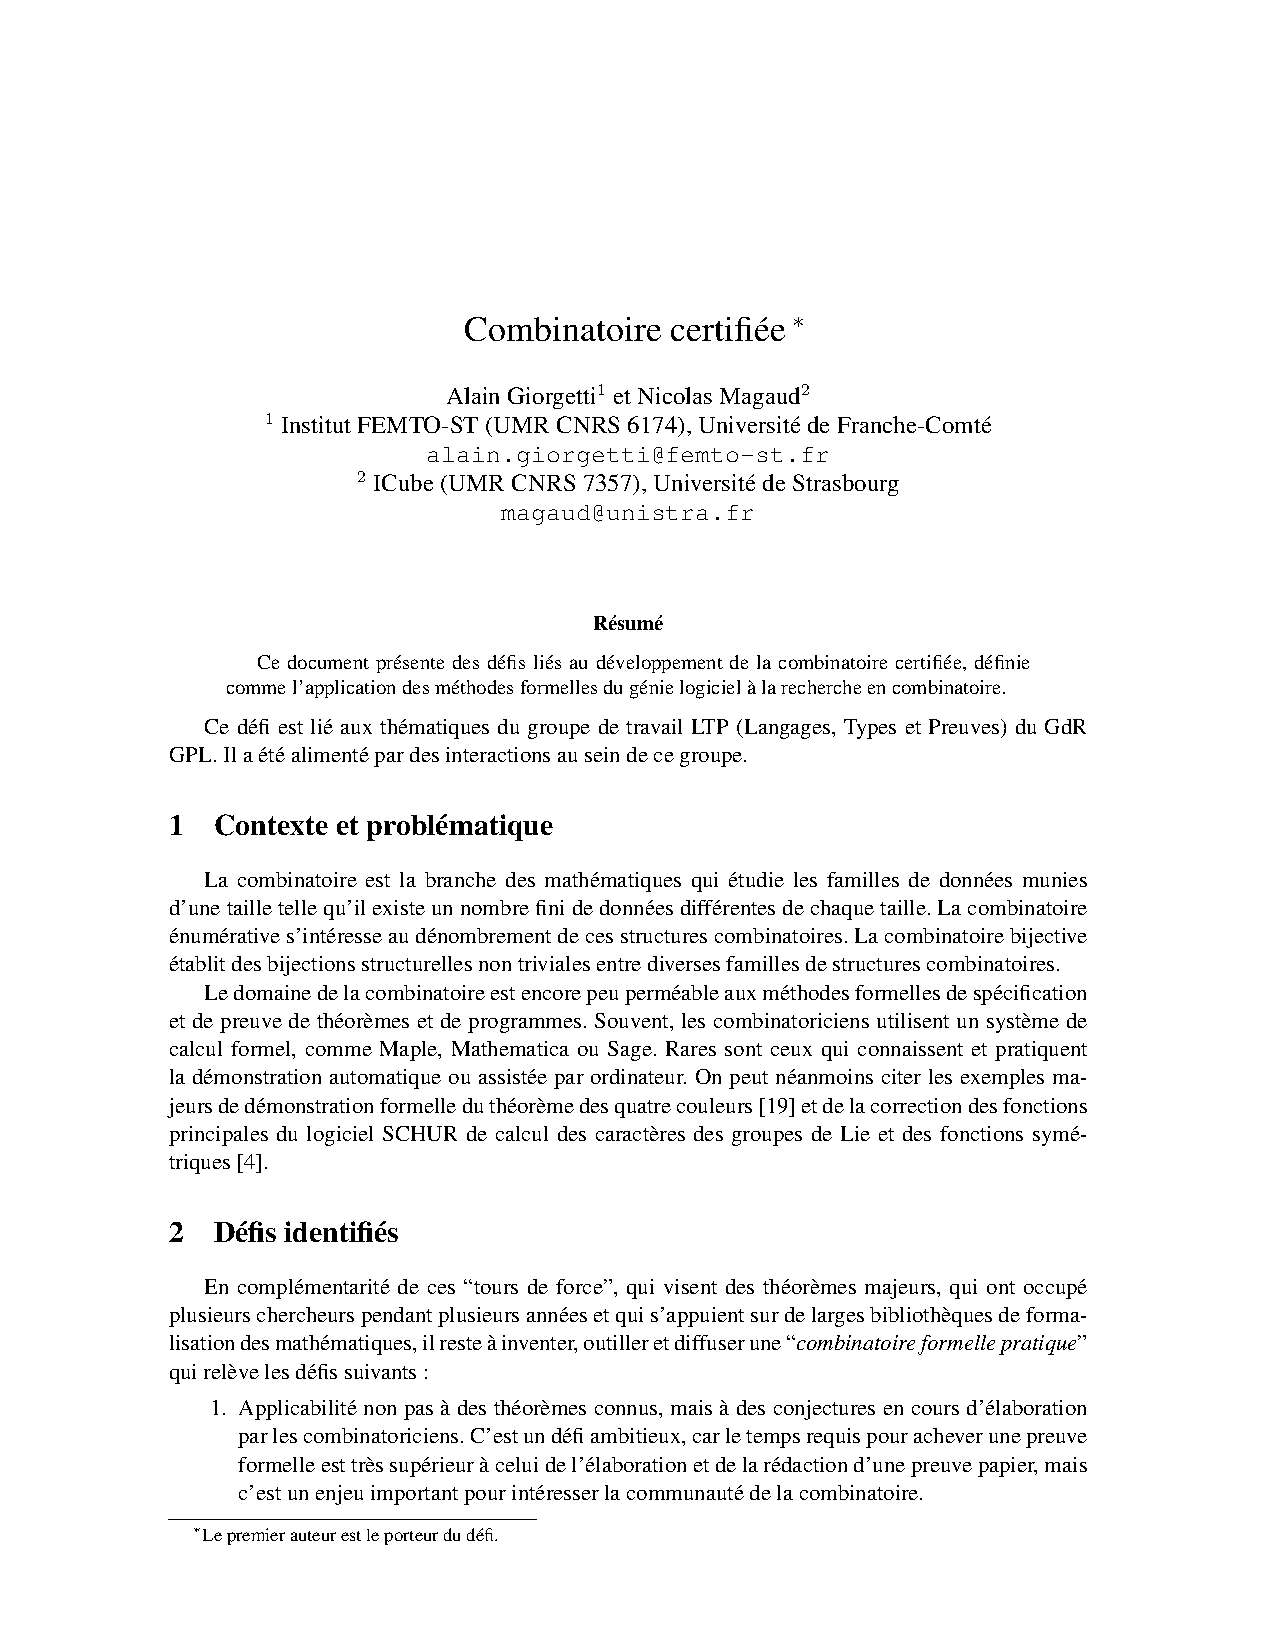
\includepdf[pages=-,pagecommand={\thispagestyle{plain}}]{Defis/combinatoire_certifiee.pdf}
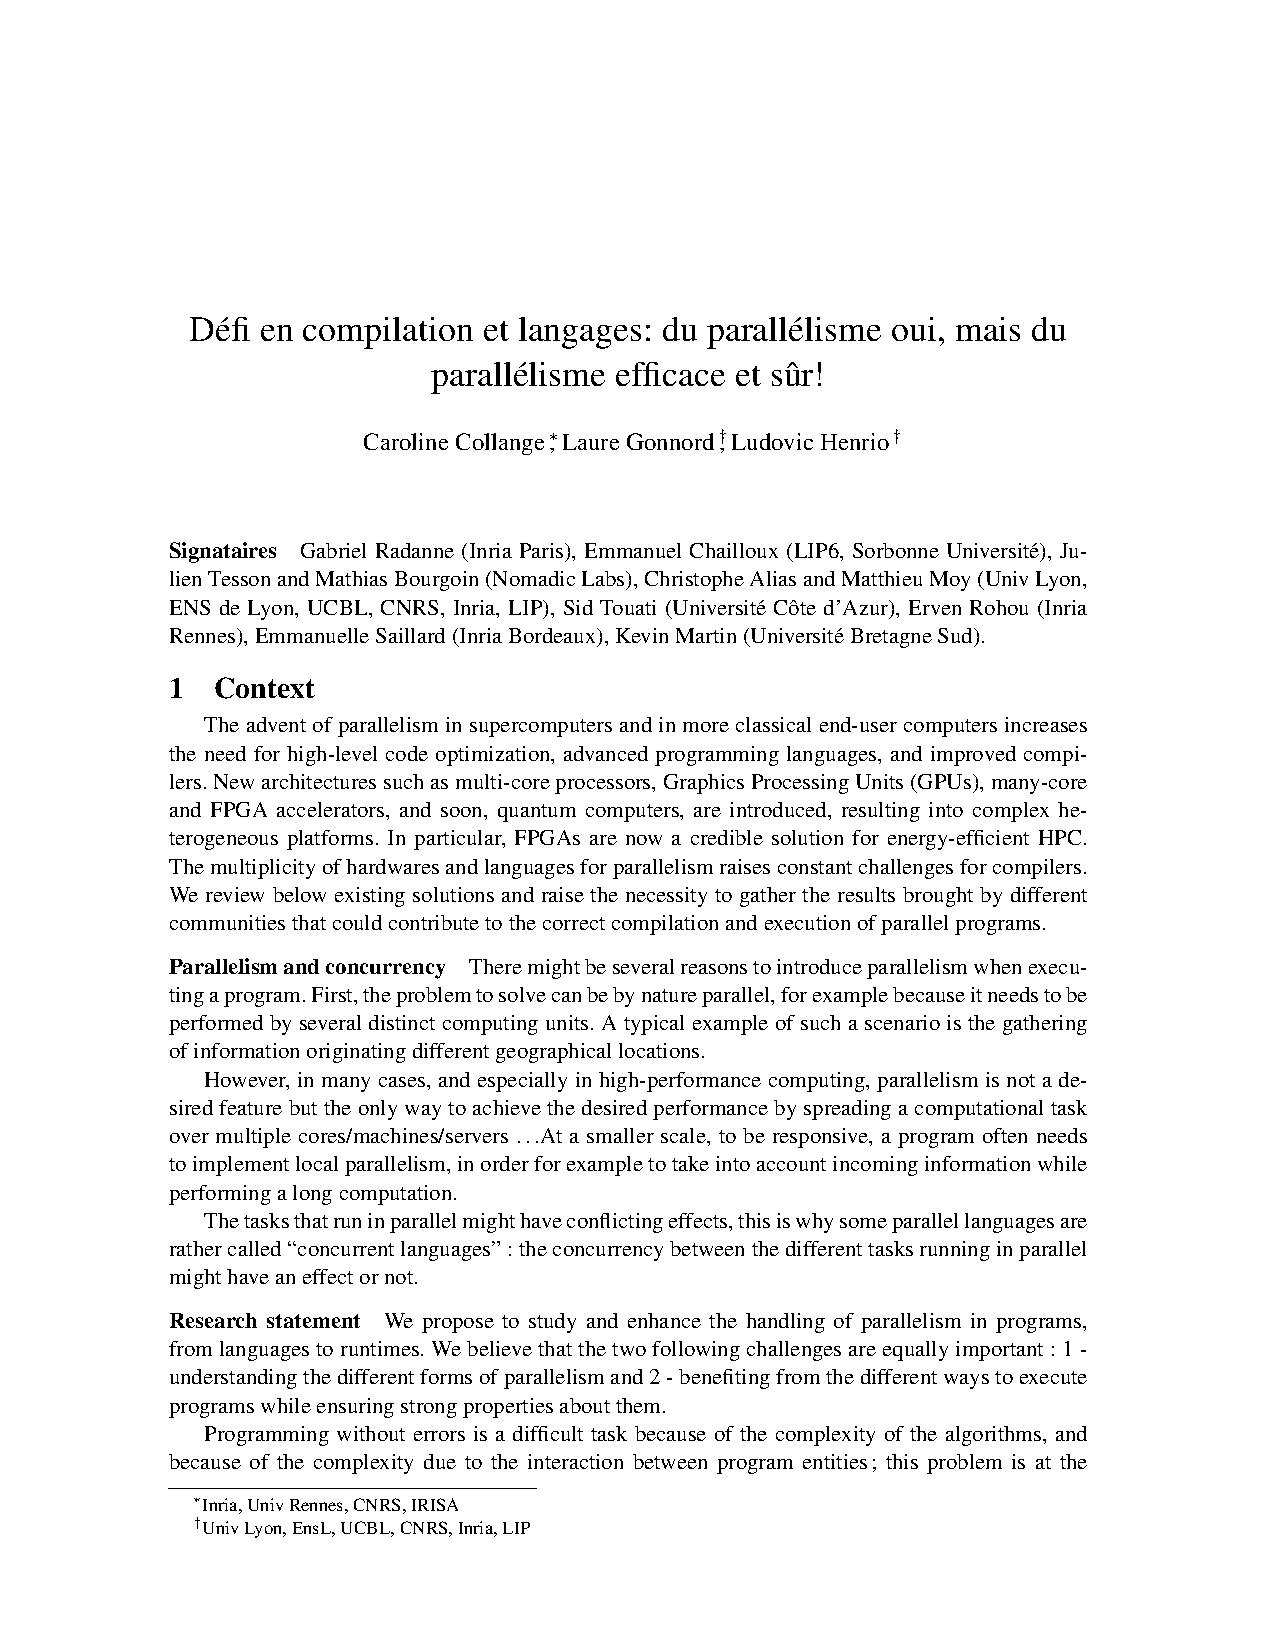
\includepdf[pages=-,pagecommand={\thispagestyle{plain}}]{Defis/Compilation_et_langages.pdf}
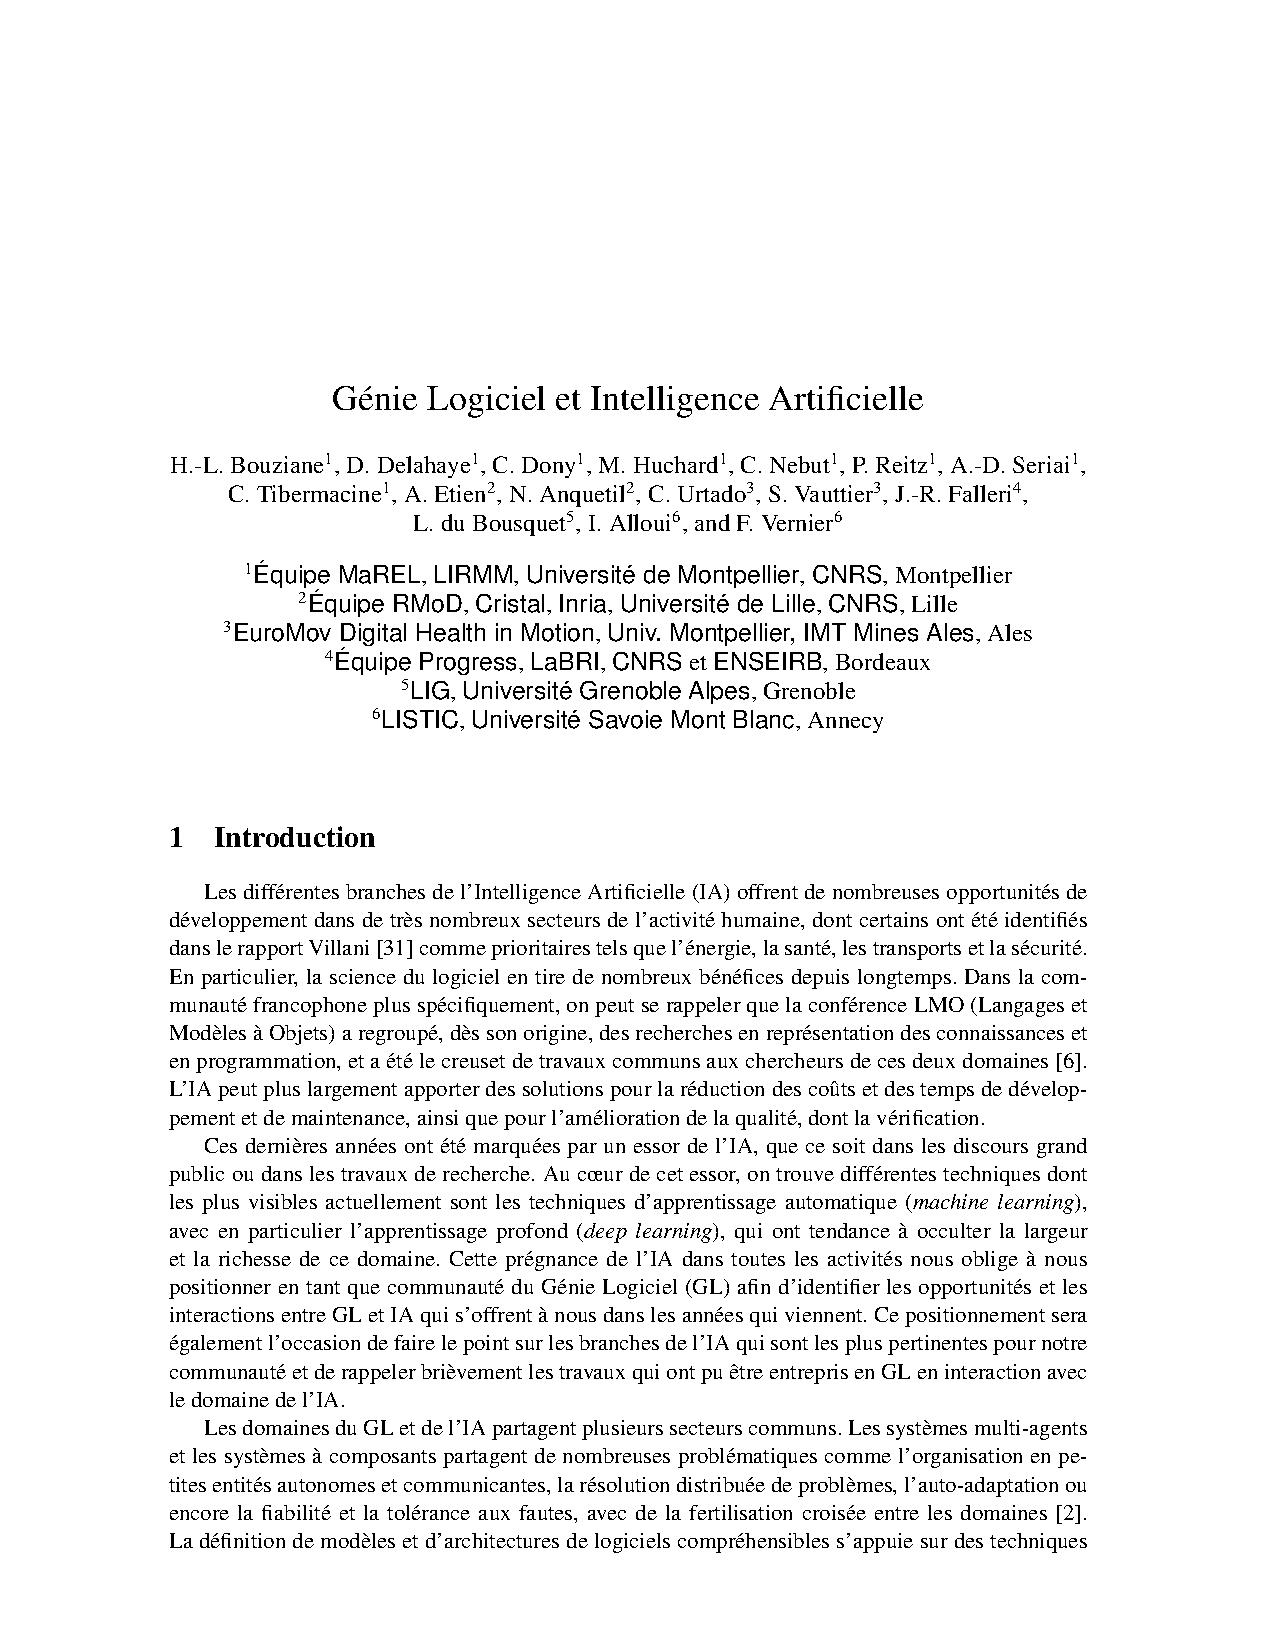
\includepdf[pages=-,pagecommand={\thispagestyle{plain}}]{Defis/Intelligence_Artificielle.pdf}
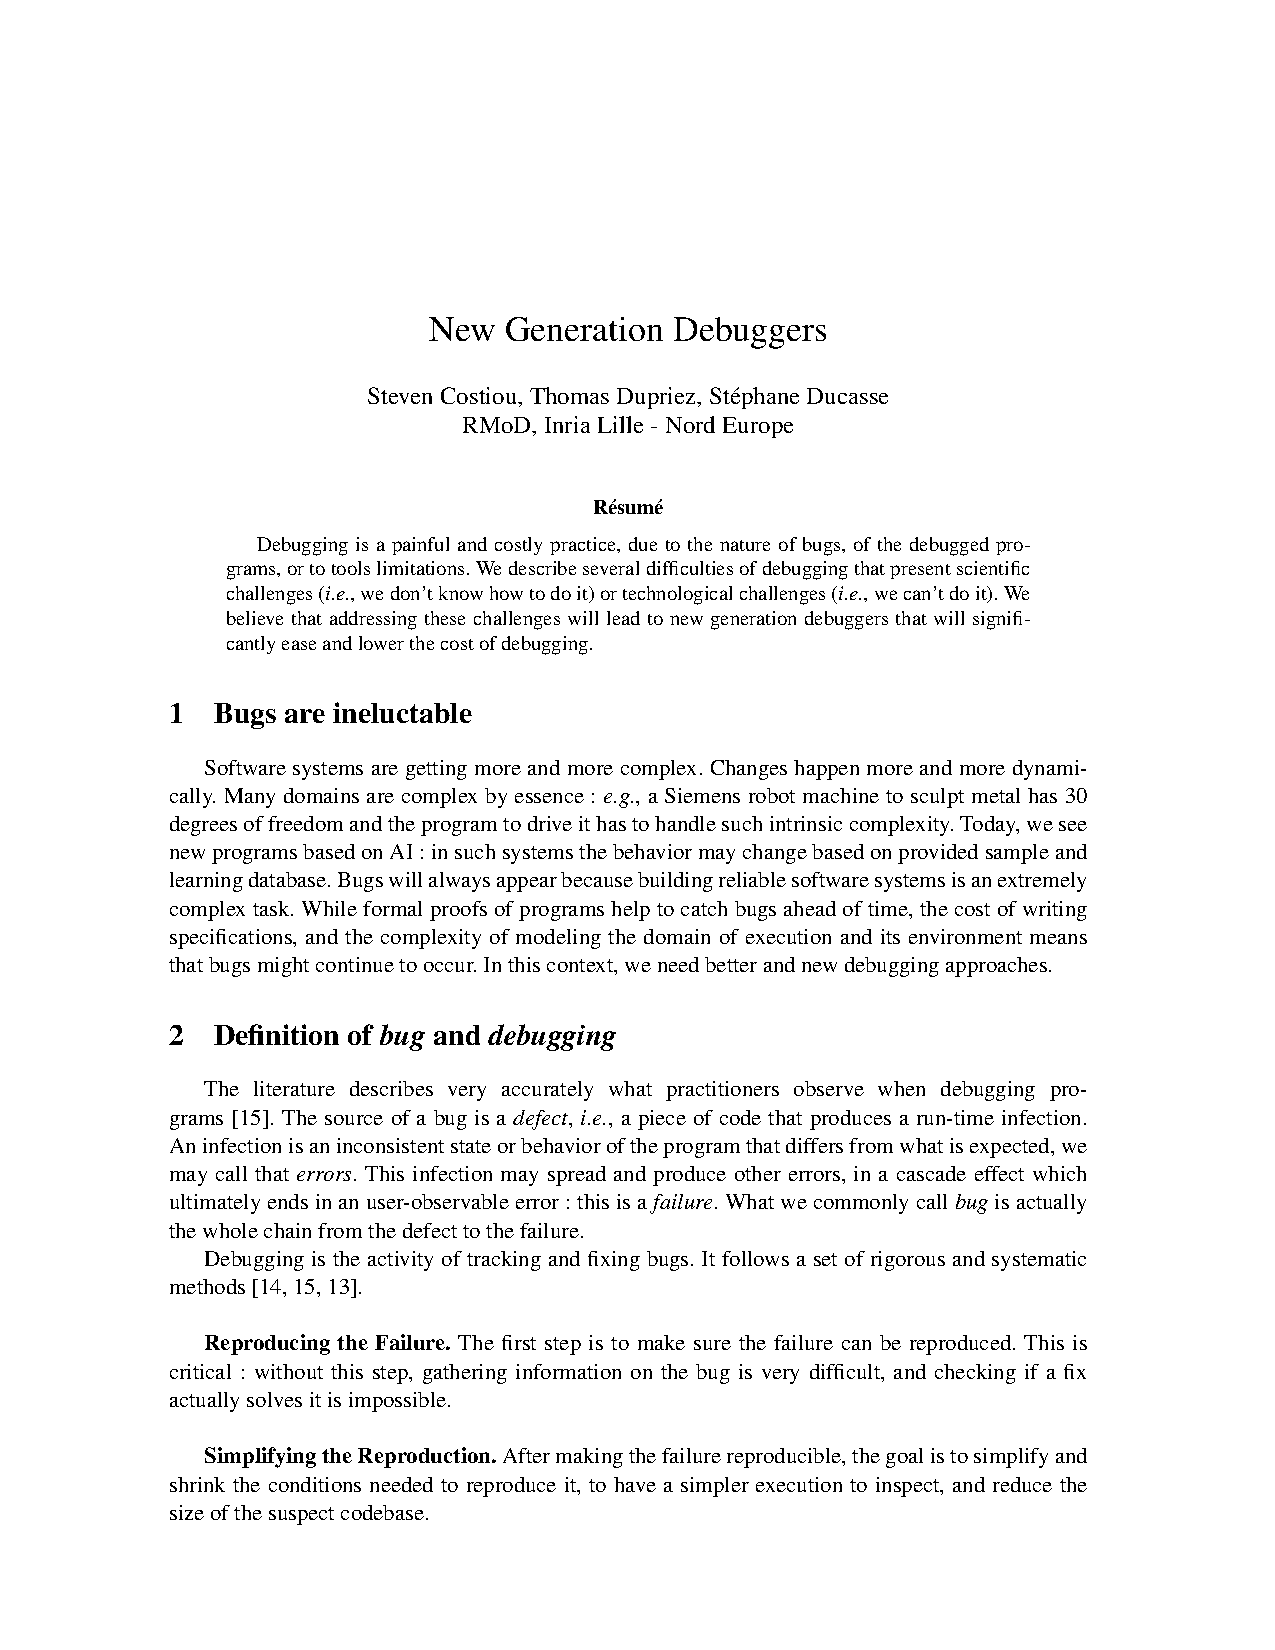
\includepdf[pages=-,pagecommand={\thispagestyle{plain}}]{Defis/New Generation Debuggers.pdf}
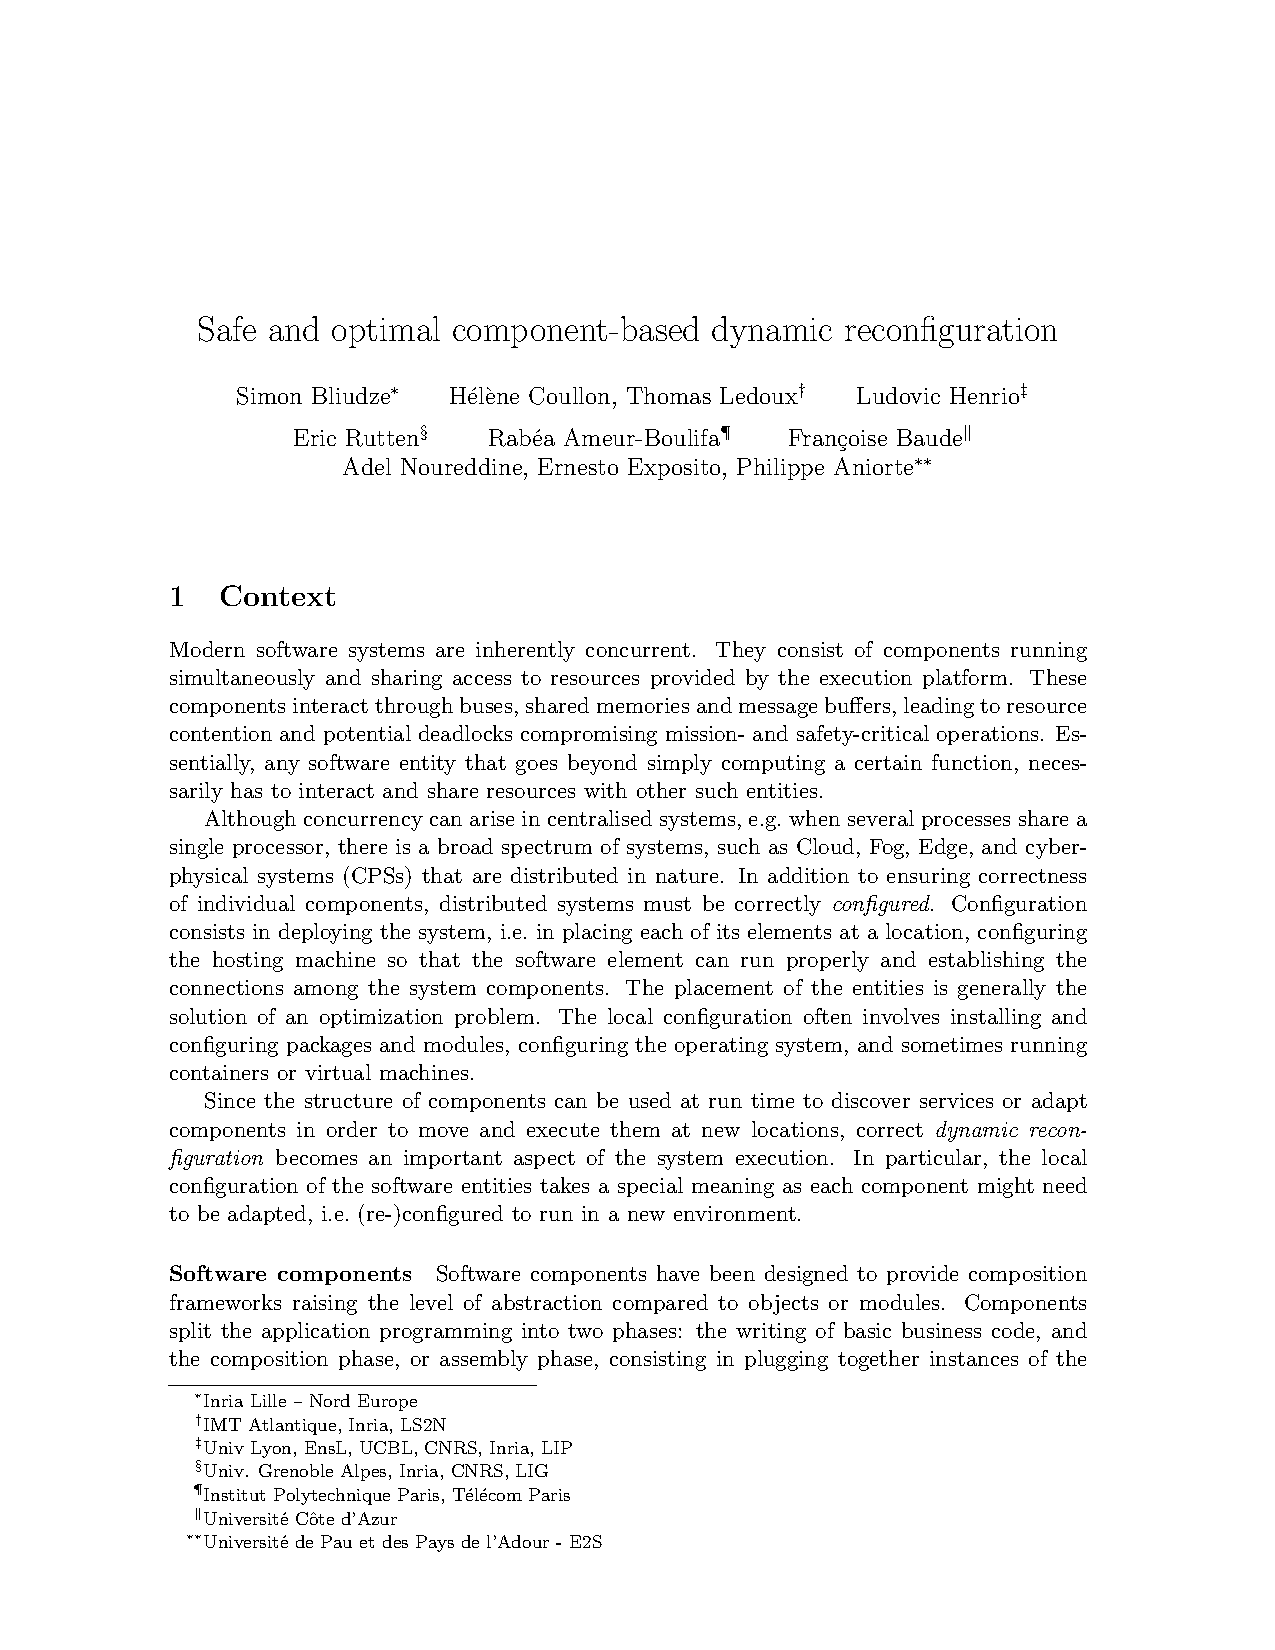
\includepdf[pages=-,pagecommand={\thispagestyle{plain}}]{Defis/Safe and optimal component-based dynamic reconfiguration.pdf}
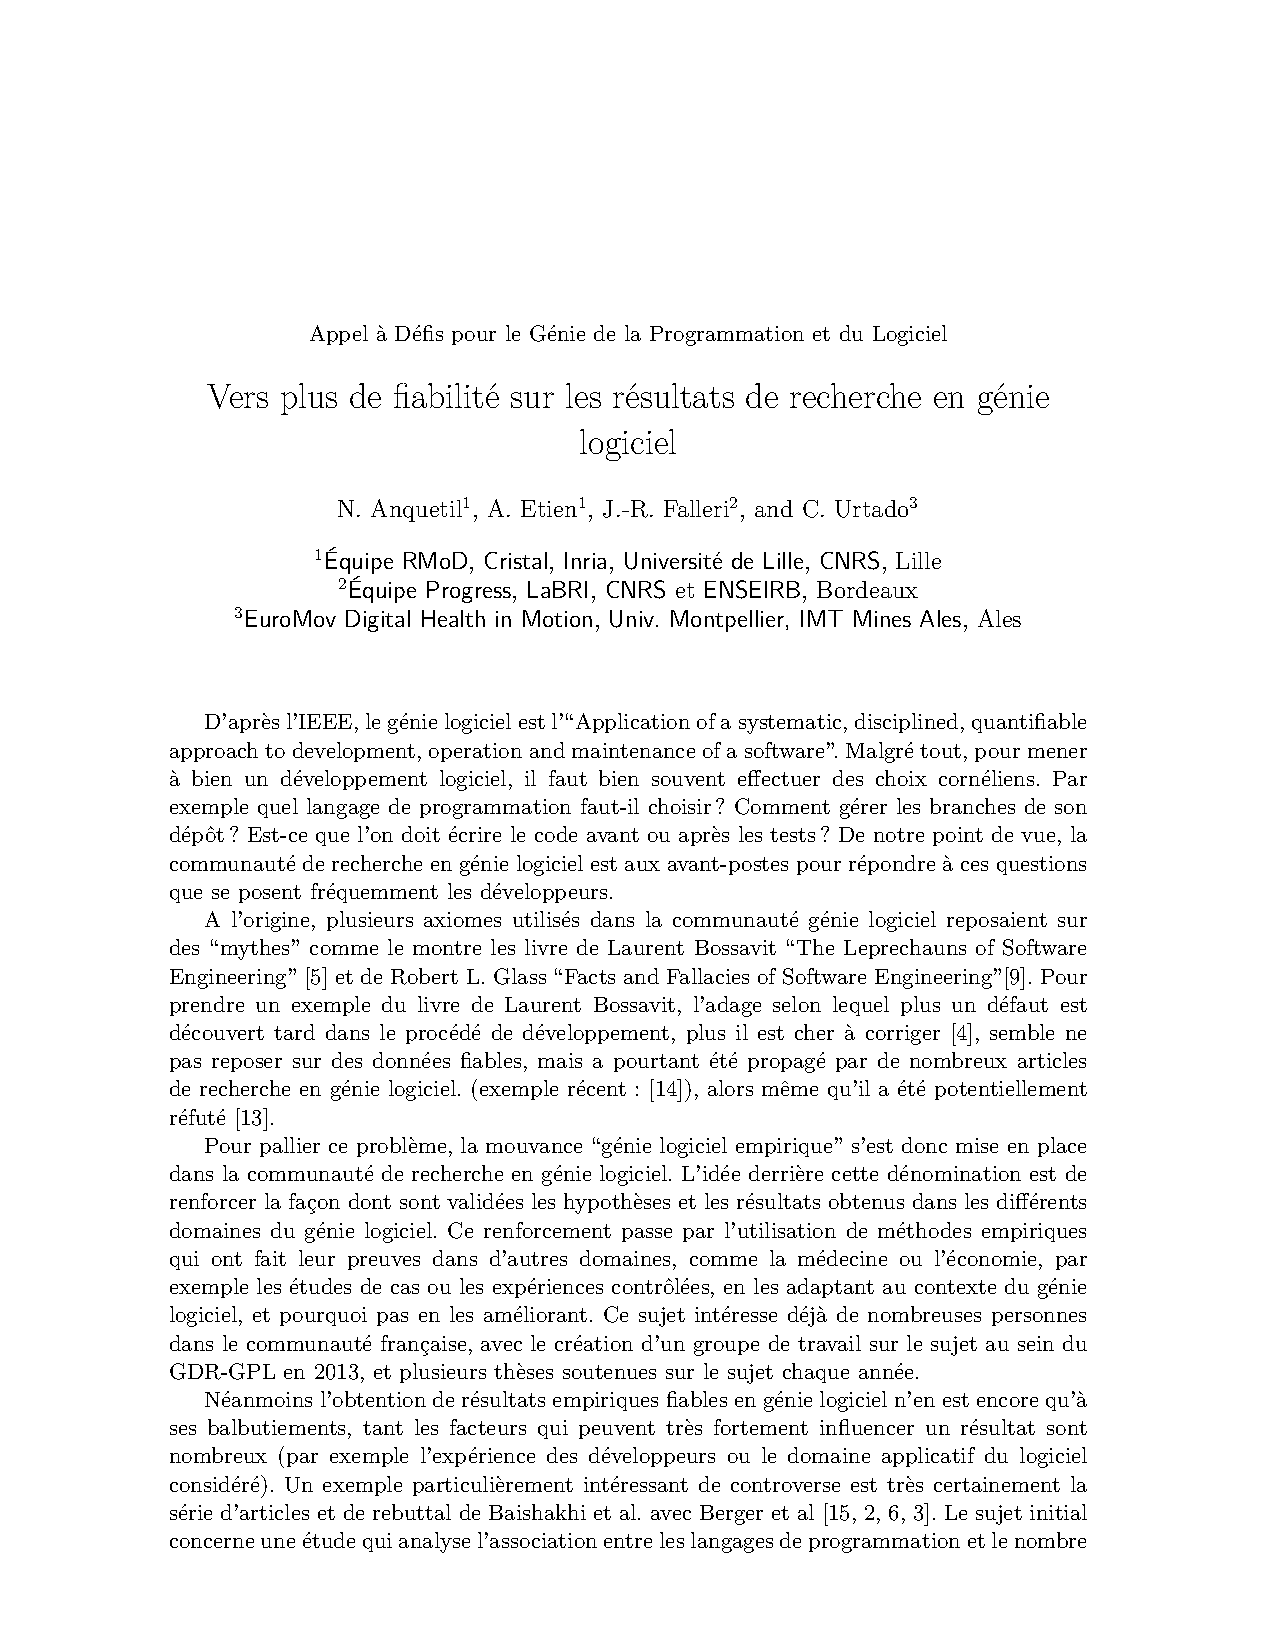
\includepdf[pages=-,pagecommand={\thispagestyle{plain}}]{Defis/Vers_plus_de_fiabilite_Res_recherche.pdf}
\end{document}
